\pagestyle{ima}
\label{ima}

\begin{textblock*}{5.625in}(0pt,0pt)%
\vspace*{-3.5cm}
\hspace*{-2.77cm}\includegraphics*[width=175.2mm]{./propagandas/IMA.pdf}
\end{textblock*}

\pagebreak %A VAGABUNDA, COLETTE

\begin{center}
\hspace*{-3.6cm}\raisebox{5cm}{\rotatebox[origin=t]{90}{\huge\Formular{\textbf{Lançamento}}}}
\hspace*{3.1cm}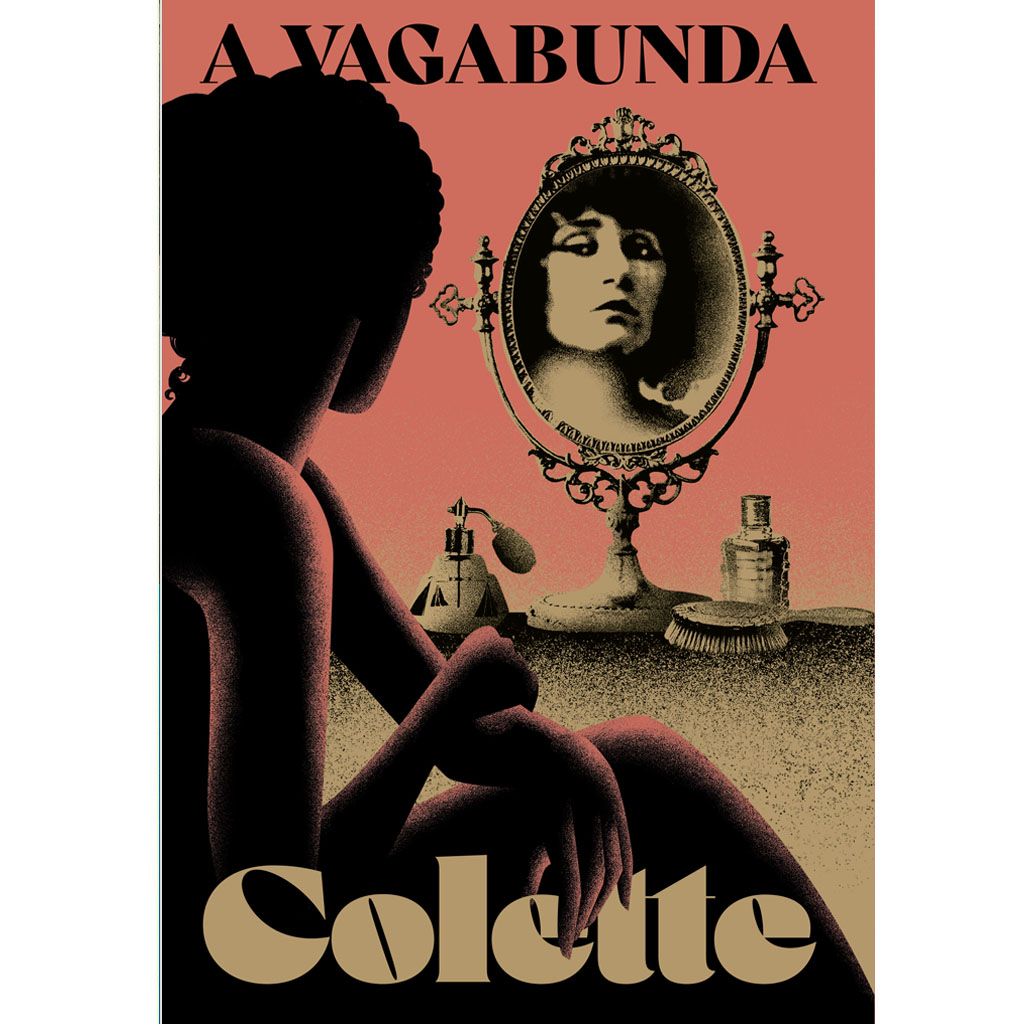
\includegraphics[width=74mm]{./grid/vagabond.jpg}
\end{center}

\hspace*{-7cm}\hrulefill\hspace*{-7cm}

\medskip

\noindent{}A indicada ao Nobel Gabrielle Sidonie Colette escreve em {\slsc{A vagabunda}} um romance passional, uma bela trajetória de libertação, tratando do pós"-divórcio da personagem, que incorpora à trajetória da protagonista Renée muito de sua própria vida pessoal. A busca pela independência de Renée, que trabalhava nos palcos do {\slsc{bas fond}} parisiense, configura “um dos mais verdadeiros retratos dos dilemas de uma mulher livre em uma sociedade dominada pelos homens” nas palavras de Angela Carter. O resultado é um clássico absoluto e um dos romances que melhor caracterizam a condição do feminino, não só do século \scalebox{.8}{XIX}.

Como a personagem, Colette foi nome presente no meio artístico da França do \scalebox{.8}{XIX}. Jornalista, atriz, mímica e escritora, lutou para livrar"-se dos grilhões que a prendiam, assim como a todas as mulheres. Seus quatro primeiros escritos, como os de Renée, foram publicados no nome de seu marido, Willy, para conseguir inserção nos círculos literários. Captando permanências e transformações, {\slsc{A vagabunda}} ainda tem muito a dizer a todas, e todos, nós.

\vfill

\hspace*{-.4cm}\begin{minipage}[c]{.5\linewidth}
\small{
{\Formular{\textbf{
\hspace*{-.1cm}\hlc[lightyellow]{Editora: Ímã}\\
Título: A vagabunda\\
Autor: Gabrielle Sidonie Colette\\ 
ISBN: 978-85-5494-616-6\\
Páginas: 286\\
Formato: 14x21cm\\
Preço: R\$ 49,90\\
Disponibilidade: Disponível
}}}}
\end{minipage}

\pagebreak 

\vspace*{1.5cm}

\noindent{}{\nohyphens{\LARGE{Um espelho todo nosso\\\noindent{}{\large\slsc{O reflexo de uma mulher que enxerga a verdade\\ em si mesma apesar da censura da sociedade}}}}}

\bigskip

\hfill{}\scalebox{.8}{DÉBORA THOMÉ}

\bigskip
\bigskip
\bigskip

Uma imagem se repete com frequência em muitas das edições e traduções de {\slsc{La Vagabonde}}, livro de 1910 da francesa Colette. Várias capas, de diferentes épocas, retratam uma mulher, com olhar desafiador, refletido diante de um espelho de camarim. A ilustração não é fortuita: se baseia em uma fotografia tirada da própria Colette durante seus anos de performance pelos palcos de Paris. 

E pensar na história de {\slsc{La Vagabonde}} é pensar em Colette, que, num ato de coragem, decide se separar do marido, um famoso editor de livros que usurpava seus textos. Vai trabalhar em um cabaré e estabelece uma relação homossexual. Ela rompe, assim, com as boas maneiras e os bons costumes da sociedade parisiense do pré"-guerras. Abandona o papel da “boa esposa”, sem grandes mágoas ou receios, para proclamar sua independência.

O mesmo caminho é o que traça Renée, a protagonista de {\slsc{A vagabunda}}. Apesar de desempenhar o papel de esposa no que era conhecido como o “casal mais interessante de Paris”, Renée decide terminar o casamento com o pintor famoso que lhe roubava seus direitos autorais. Recusa"-se seguir como esposa traída e vai experimentar os riscos de viver livre de um homem. A cidade que ambienta a trama era a moderna Paris do início do século \scalebox{.8}{XX}: 1906 para Colette; 1910 para Renée. Naquela ocasião às “mulheres corretas” apenas cabia cuidar de suas casas e filhos. Havia, sim, muitos artistas e cabarés, mas o direito a não ter um cônjuge era exclusivo dos homens. A sociedade francesa ainda destilava preconceito sobre mulheres que optavam por viver sozinhas, as “damas desacompanhadas“, ainda mais as que se sustentavam fazendo arte.

Se Colette tinha algum medo, fez questão de traçar uma vida na qual o enfrentou bem. Casou"-se e divorciou"-se quantas vezes quis, morreu rompida com a Igreja e acabou enterrada com honras de Estado. Tampouco parece que cedeu ao medo de sua personagem Renée: seus momentos de temor da solidão na história parecem quase forjados. A liberdade que então passou a experimentar, mesmo com pouco dinheiro e muito cansaço, compensava as vastas incertezas. Era livre para não precisar prestar contas a ninguém. Às mulheres estava destinado o espaço doméstico: uma boa esposa devia estar condenada na sua casa, cumprindo os desejos de sua família, temente a Deus e a seu marido. Enquanto isso, aos homens era permitido transitar entre diferentes mundos, fazer escolhas, ter liberdade dentro e fora de suas casas. Mais de um século depois de Renée ter surgido ao mundo como a vagabunda, a história escrita por Colette, versão romanceada de sua própria vida, permanece absolutamente atual.

Desde 1910, ano em que o livro foi publicado na França, o feminismo deu largos passos. O voto das mulheres, resultante dos esforços das sufragistas em todo o mundo, foi aprovado na França após a Segunda Guerra, em 1945 (o Brasil o aprovou antes, em 1932). Quatro anos depois, em 1949, veio a público a primeira edição da “bíblia” do movimento feminista, {\slsc{O segundo sexo}}, de Simone de Beauvoir.

Muitas ações tiveram lugar após esses primeiros marcos, e as feministas seguiram em busca de diferentes tipos de liberação e ampliação de direitos. Houve avanços expressivos quanto aos direitos políticos, civis e sociais --- mulheres hoje têm autonomia em suas famílias, e o divórcio é letra corrente na maioria dos países. No entanto, resistiu a todas essas mudanças a ideia de que a mulher deve se casar, e sobretudo ter filhos. A perspectiva é de uma vida em pares. E, nesse sentido, mesmo transpostos ao Brasil atual, os dilemas de Renée ainda soam bastante verossímeis. 

A nossa “vagabunda” --- que no equivalente em francês {\slsc{vagabonde}} mantém somente o sentido original, de quem vagueia por aí --- segue sendo a mulher libertina, cuja alcunha vem da quantidade de homens com quem se relaciona. A expectativa de que o bom casamento é o que salva as mulheres dos infortúnios da vida persiste em Terra Brasilis. Aos maridos, o sustento financeiro das mulheres; às esposas, a submissão, o trabalho doméstico não remunerado e o sustento emocional dos homens.

Mesmo decidindo agir de acordo com sua verdade, em determinado momento Renée escuta de seus familiares: “E que é que você queria, minha filha?” Como leitoras, é bem clara a resposta: a protagonista queria mais da vida. Diante de uma maré de resistência a uma sociedade acostumada a funcionar de tal forma, Renée se dá conta de sua sujeição e se rebela. Ela mantém seus propósitos firmes a despeito dos custos que paga. Do risco da fome, do quarto de pensão, da viagem na segunda classe. O ônus de ser solteira lhe trouxe a vantagem de ser ela a única responsável por suas próprias escolhas. Renée, mais uma vez, tal e qual Colette. 

A protagonista vagabunda é uma feminista do seu tempo, à sua moda. É principalmente alguém que conseguiu desarmar a regra geral quando viu sua liberdade e seus direitos ameaçados. Sua grandeza está em questionar o que é dado como norma, como o normal. Até o ciúme, que vive servindo na narrativa universal como exemplo de prova de amor, perde seu lugar no pedestal. 

Ao contar a história de Renée, Colette chega a flertar com o romance. Contudo, opta por romper com a tradição de uma literatura que sempre atribuía às personagens femininas o papel de donzelas chorosas em busca um príncipe salvador. Ao contrário disso, sua novela é escrita e narrada por mulheres que questionam o papel social a elas atribuído.

Ainda que se trate de outro tipo de inserção política, em alguns momentos, o ritmo de {\slsc{A vagabunda}} lembra trechos e dinâmicas de {\slsc{Parque industrial}}, obra brasileira de 1936, assinada por Mara Lobo, pseudônimo de Patrícia Galvão, a Pagu. A vagabunda Renée, por sua vez, também traz ares da compositora Chiquinha Gonzaga, que rompe com tudo e todos para viver com sua música.

Essas expoentes mais ou menos contemporâneas --- Pagu, Colette e Chiquinha --- assemelham"-se sobretudo por um motivo: todas enfrentaram os valores patriarcais tentando estabelecer novos padrões para a mulher nas sociedades em que viviam. A protagonista Renée também compõe este quadro. A luta individual de cada uma dessas personagens reais e fictícias acabou se tornando exemplar do que passavam (e passam) muitas mulheres: a esfera pessoal lhes é política. Portanto, para que a rebelião ocorra, dando início uma nova ordem, é preciso romper com a “segurança imbecil das mulheres que são amadas [\ldots{}] cujos desejos são satisfeitos.”

No livro {\slsc{Performing Women and Modern Literary Culture in Latin America}}, a autora Vicky Unruh, professora emérita da Universidade do Kansas (\scalebox{.8}{EUA}), discorre sobre como muitas mulheres latino"-americanas no início do século \scalebox{.8}{XX} transformaram sua experiência concreta de vida em performances, como estratégia para poderem participar de uma cultura literária na qual não eram bem"-vindas. Vida e proposta artística se confundiam. Entretanto se, por um lado, as mulheres tinham mais dificuldade de ocupar espaços devido às barreiras de gênero, por outro, justamente porque sua simples presença já afrontava o {\slsc{status quo}}, elas tinham mais facilidade para criarem novas realidades. As artistas performáticas, como Renée e Colette, transitavam entre a esfera pública e a privada; nos palcos e na escrita. Fosse na Europa ou nas Américas, refletiam na arte aquilo que viviam em suas vidas.

Colette, afinal, sabe que só tem um jeito de propor a transformação: fazendo com que Renée vença suas próprias fragilidades, aquelas que foram ensinadas a ela e a maioria das mulheres desde muito cedo. Renée, por sua vez, obedece aos desígnios da autora que conduz seus passos. Sem questionar, entende seu destino como vagabunda e não cede ao papel esperado, nem a um roteiro padrão. Estabelece um pacto firme, irredutível, com a sua independência, com a sua liberdade.\footnote[1]{Adaptado do posfácio do livro {\slsc{A vagabunda}}.}


\pagebreak %BIOGRAFIA DO LÍNGUA


\begin{center}
\hspace*{.5cm}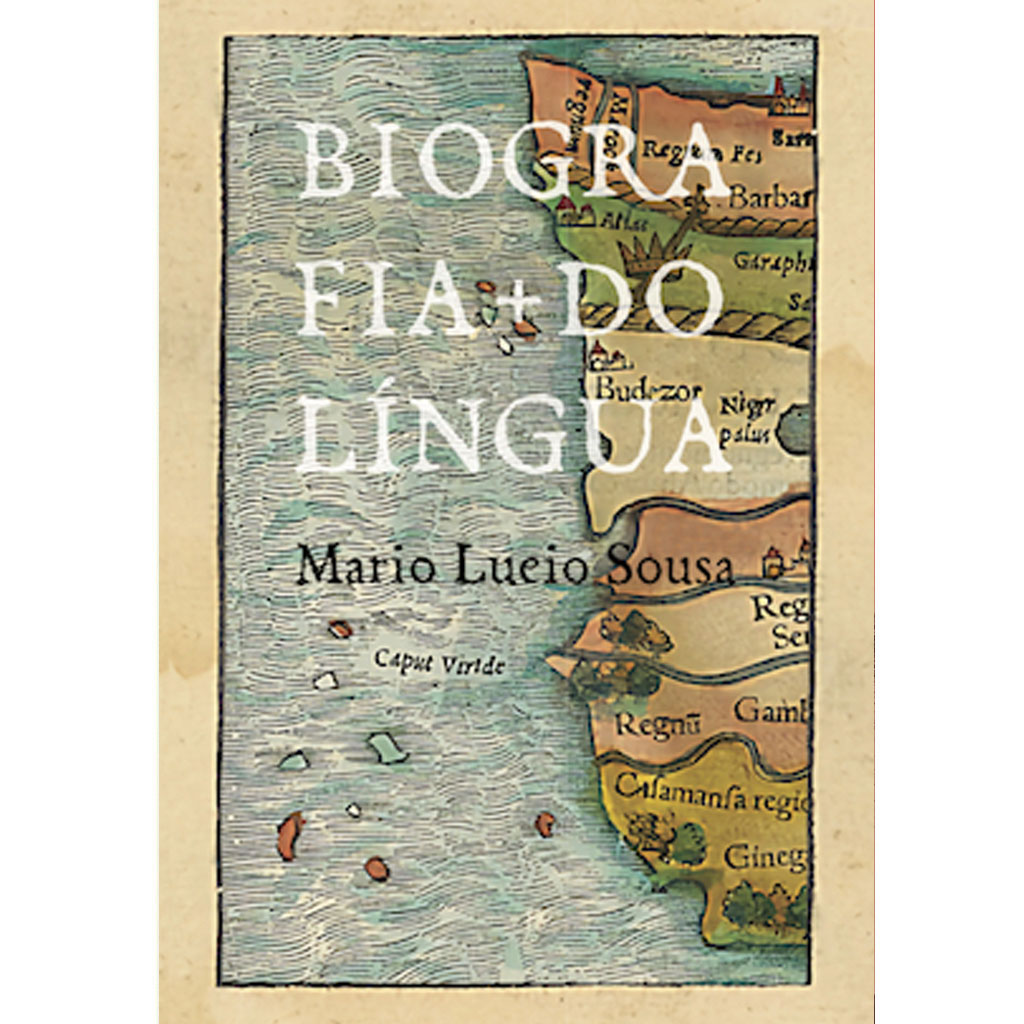
\includegraphics[width=74mm]{./grid/lingua.jpg}
\end{center}

\hspace*{-7cm}\hrulefill\hspace*{-7cm}

\medskip

\noindent{}O último desejo de um condenado à morte é contar a vida do Língua, escravo prodigioso obrigado a uma das mais degradantes atividades que um escravo poderia exercer: traduzir as falas dos brancos nos navios negreiros para os povos da África. Enquanto é contada a fabulosa biografia, pessoas se aproximam para ouvir e acabam por escrever juntas a história de um lugar, atravessando colônia, de independência e revolução.

A ficção foi inspirada, segundo o autor cabo"-verdiano Mario Lucio Sousa, em um homem real, talvez o único neste mundo que viveu o colonialismo, a escravatura, a abolição, a guerra da independência, a independência, a ocupação, o capitalismo, o imperialismo e o comunismo, sucessivamente e num mesmo lugar, entrevistado pelo etnólogo Miguel Barnet em 1963. Esse homem tinha 104 anos e dizia chamar"-se Esteban Montejo. {\slsc{Biografia do Língua}} é, portanto, um livro em que a personagem central é a própria maravilha de se contar histórias.

\vfill

\hspace*{-.4cm}\begin{minipage}[c]{.5\linewidth}
\small{
{\Formular{\textbf{
\hspace*{-.1cm}\hlc[lightyellow]{Editora: Ímã}\\
Título: Biografia do Língua\\
Autor: Mario Lucio Sousa\\ 
ISBN: 978-85-5494-612-8\\
Páginas: 302\\
Formato: 14x21cm\\
Preço: R\$ 54,00\\
Disponibilidade: 17/07/2020
}}}}
\end{minipage}

\pagebreak %A LUTA, CARMEN DOLORES


\begin{center}
\hspace*{-3.6cm}\raisebox{5cm}{\rotatebox[origin=t]{90}{\huge\Formular{\textbf{Lançamento}}}}
\hspace*{3.1cm}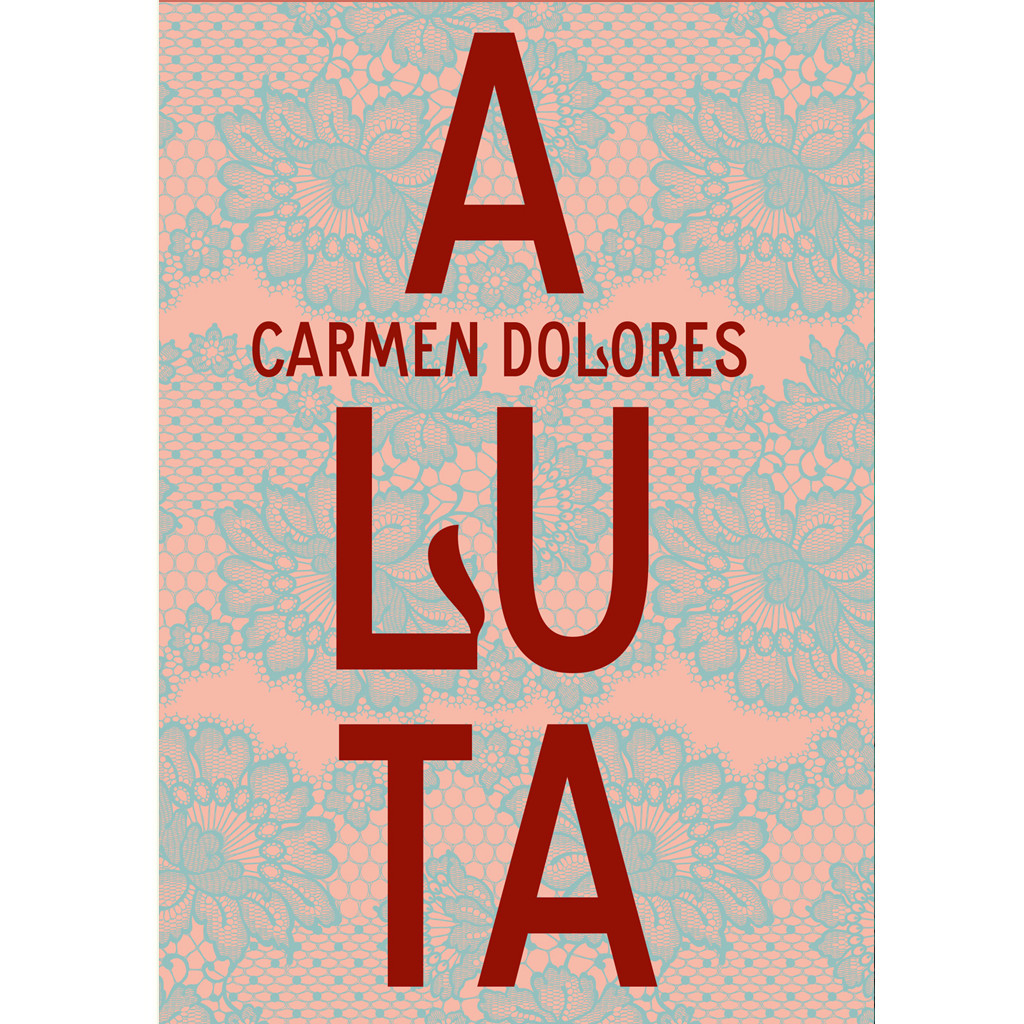
\includegraphics[width=74mm]{./grid/luta.jpg}
\end{center}

\hspace*{-7cm}\hrulefill\hspace*{-7cm}

\medskip

\noindent{}Cecília se rebela contra sua vida na “masmorra” das amarras patriarcais de um casamento insosso e do duplo jugo da mãe ambiciosa e da sogra conservadora: a casa que divide com a sogra ciumenta, o marido insípido e dois filhinhos. Essa “Madame Bovary da rua das Marrecas sonhava com uma existência maior, a independência da mulher elegante e rica, que sai só, vai a teatros e alimenta a corte ardente de muitos admiradores”.

Um retrato desabusado do que era ser mulher em uma sociedade (ainda mais) dominada pelos homens, escrito por uma das mais corajosas e influentes jornalistas do começo do século \scalebox{.8}{XX}, convenientemente “esquecida” entre os grandes escritores brasileiros. Carmen Dolores é o pseudônimo mais conhecido de Emília Moncorvo Bandeira de Melo, uma das mais representativas e influentes escritoras do início do século \scalebox{.8}{XX}, pioneira na luta dos direitos femininos. Em uma época em que mulheres não podiam votar, Emília tratou de temas com escrita incisiva e corajosa como o direito ao divórcio, educação e acesso igualitário ao mercado de trabalho. 


\vfill

\hspace*{-.4cm}\begin{minipage}[c]{.5\linewidth}
\small{
{\Formular{\textbf{
\hspace*{-.1cm}\hlc[lightyellow]{Editora: Ímã}\\
Título: A luta\\
Autor: Carmen Dolores\\ 
ISBN: 978-85-5494-620-3\\
Páginas: 180\\
Formato: 14x21cm\\
Preço: R\$ 42,90\\
Disponibilidade: 17/07/2020
}}}}
\end{minipage}

\pagebreak
\pagestyle{imacat}

\begin{multicols}{2}
\begin{enumerate}
\raggedright\nohyphens{
\item Marcelino, {\Formular{\textbf{Godofredo De Oliveira Neto}}}
\item Desamores da portuguesa, {\Formular{\textbf{Marta Barbosa Stephens}}}
\item Clube da esquina - Milton Nascimento e Lô Borges, {\Formular{\textbf{Milton Nascimento; Lô Borges; Charles Gavin}}}
\item Parasito, {\Formular{\textbf{Andrea Rangel}}}
\item Academia de danças - Egberto Gismonti, {\Formular{\textbf{Egberto Gismonti; Charles Gavin}}}
\item Secos \& Molhados, {\Formular{\textbf{Ney Matogrosso; Gerson Conrad; Charles Gavin}}}
\item 100 dias em Paris, {\Formular{\textbf{Tania Carvalho}}}
\item Perdidas, {\Formular{\textbf{Andrea del Fuego; Edney Silvestre; Henrique Rodrigues; Marcelo Moutinho; Marta Barbosa Stephens; Martha Batalha; Kátia Bandeira de Mello  Gerlach; Alexandre Staut}}} 
\item Rosa de ouro - Aracy Côrtes e Clementina de Jesus, {\Formular{\textbf{Hemínio Bello de Carvalho; Paulinho da Viola; Elton Medeiros; Charles Gavin}}}
\item Chico Buarque para todos, {\Formular{\textbf{Regina Zappa}}}
\item Galos de briga - João Bosco, {\Formular{\textbf{João Bosco; Charles Gavin}}}
\item Quem é quem - João Donato, {\Formular{\textbf{João Donato; Marcos Valle; Charles Gavin}}}
\item Dois - Legião Urbana, {\Formular{\textbf{Dado Villa-Lobos; Marcelo Bonfá; Charles Gavin}}}
\item Mulheres que mordem, {\Formular{\textbf{Beatriz Leal}}}
\item Nervos de aço - Paulinho da Viola, {\Formular{\textbf{Paulinho da Viola; Charles Gavin; Monarco}}}
\item Sociedade dividida, {\Formular{\textbf{Raphael Lima}}}
\item Estudando o samba - Tom Zé, {\Formular{\textbf{Tom Zé; Charles Gavin}}}
\item Reprograme, {\Formular{\textbf{Cory Doctorow; Nina Simon; Jane Finnis; Luis Marcelo Mendes}}}
\item Como o Botafogo conquistou a China, {\Formular{\textbf{Bruno Porto}}}
\item A peleja do diabo com o dono do céu - Zé Ramalho, {\Formular{\textbf{Zé Ramalho; Charles Gavin}}}
\item A árvore oca, {\Formular{\textbf{Mauricio Vieira}}}
\item A morte visita Lisboa, {\Formular{\textbf{Fernando Perdigão}}}
\item Biografia do Língua, {\Formular{\textbf{Mario Lucio Sousa}}}
\item 100 dias em Lisboa, {\Formular{\textbf{Tania Carvalho}}}
\item A vagabunda, {\Formular{\textbf{Sidonie Gabrielle Colette}}}
}
\end{enumerate}
\end{multicols}

\pagebreak

%\hspace{.5cm}
%
%\begin{center}
%\hspace*{-.5cm}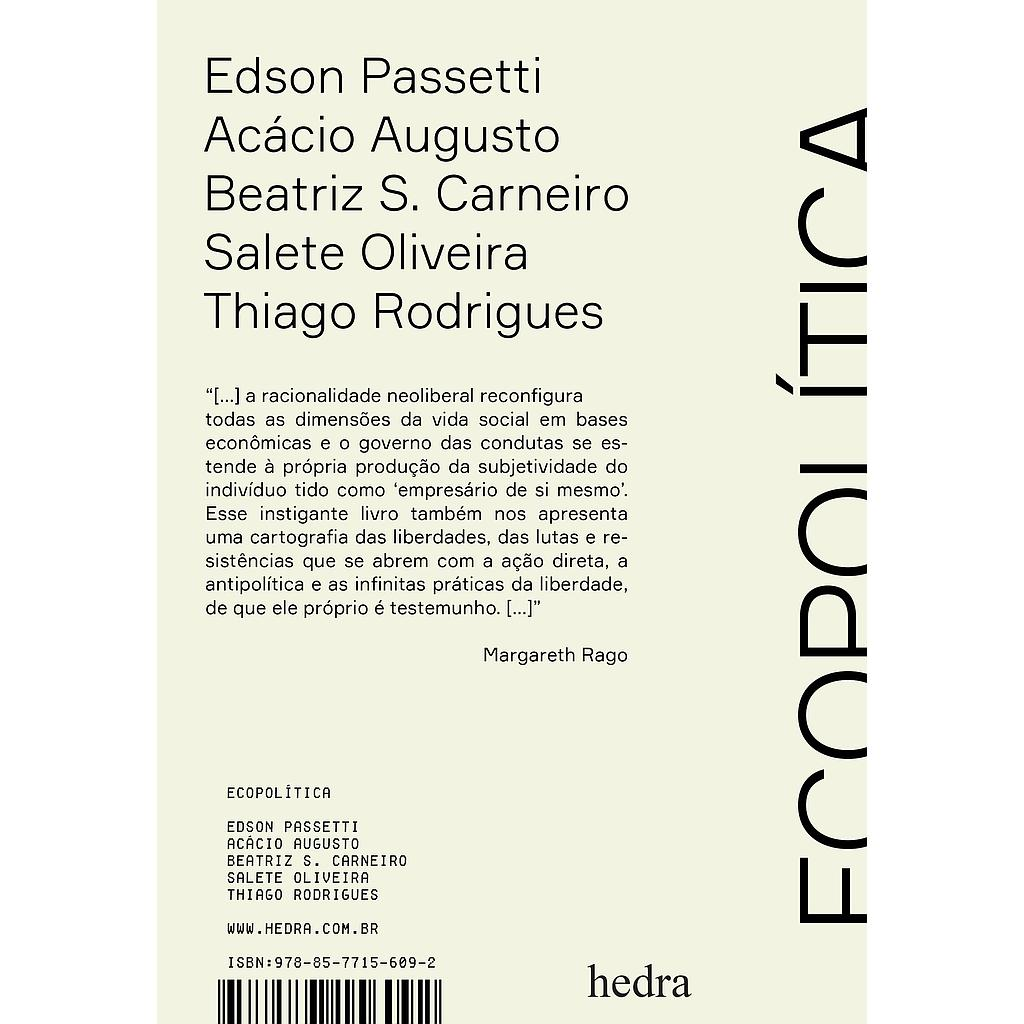
\includegraphics[width=70mm]{eco.jpeg}
%%\hspace*{6cm}\raisebox{2cm}{\rotatebox[origin=t]{90}{\Formular{\textbf{Lançamento}}}}
%\end{center}
%
%\hspace*{-2cm}\_\_\_\_\_\_\_\_\_\_\_\_\_\_\_\_\_\_\_\_\_\_\_\_\_\_\_\_\_\_\_\_\_\_\_\_\_\_\%_\_\_\_\_\_\_\_\_\_\_\_\_\_\_\_\_\_\_\_\_\_\_\_\_\_\_\_\_\_\_\_\_\_\_\_
%
%\medskip
%
%\noindent{}Lorem ipsum dolor sit amet, consectetur adipiscing elit.
%Donec sodales tortor a purus accumsan, ut ultricies purus
%maximus. Aliquam bibendum consequat mi, sed commo-
%do velit pellentesque id. Vivamus ultricies ligula in semper
%sagittis. Donec mollis odio in lectus tristique, sed convallis
%est interdum. Cras eget sem condimentum, pretium purus
%eu, auctor.
%
%\hspace{.5cm}
%
%\hspace*{-.4cm}\begin{minipage}[c]{0.45\linewidth}
%\small{
%{\Formular{\textbf{
%\hspace*{-.1cm}Título: Ecopolítica\\
%Autor: Edson Passetti\\ 
%Editora: Hedra\\
%Páginas: 476\\
%Formato: 23x16cm\\
%Preço: R\$ 79,90\\
%}}}}
%\end{minipage}
%\begin{minipage}[c]{0.50\linewidth}
%\small{Lorem ipsum dolor sit amet, consectetur adipiscing elit. onec sodales tortor a purus accumsan, ut ultricies. Lorem ipsum dolor sit amet, %consectetur adipiscing elit. Lorem ipsum dolor sit amet. Lorem ipsum dolor sit amet.} 
%\end{minipage}